\documentclass{article}
\usepackage{amsmath}
\usepackage{listings}
\usepackage{xcolor}
\usepackage{graphicx}
\usepackage{geometry}
\usepackage{hyperref}
\usepackage{tikz}
\usetikzlibrary{trees, positioning}
\geometry{margin=1in}

\title{Dynamic Programming}
\author{}
\date{}

\definecolor{codegray}{rgb}{0.5,0.5,0.5}
\definecolor{backcolour}{rgb}{0.95,0.95,0.92}

\lstdefinestyle{cppstyle}{
  backgroundcolor=\color{backcolour},
  commentstyle=\color{codegray},
  keywordstyle=\color{blue},
  numberstyle=\tiny\color{codegray},
  stringstyle=\color{red},
  basicstyle=\ttfamily\footnotesize,
  breakatwhitespace=false,
  breaklines=true,
  captionpos=b,
  keepspaces=true,
  numbers=none,
  numbersep=5pt,
  showspaces=false,
  showstringspaces=false,
  showtabs=false,
  tabsize=2,
  language=C++
}

\begin{document}

\maketitle

Algorithm design strategies seen thus far:
\begin{itemize}
    \item Brute force — exhaustively consider through all possibilities
    \item Divide and conquer — examples: binary search, mergesort, quicksort
    \item Greedy algorithm — examples: Prim's algorithm for minimum spanning tree, Dijkstra's algorithm for single source shortest path
    \item Dynamic programming — this lecture
\end{itemize}

\section{Definitions}

Dynamic Programming is an algorithmic paradigm: It is used when the solution can be recursively described in terms of solutions to subproblems (optimal substructure).

Unlike divide and conquer, where subproblems are independent and solved separately, dynamic programming applies when subproblems \textit{overlap}—i.e., the same subproblems recur multiple times. DP solves each subproblem once and stores the result for reuse, thereby avoiding redundant computation.

\textbf{Memoization:} Algorithm finds solutions to subproblems and stores them in memory for later use.  
More efficient than brute-force methods, which solve the same subproblems over and over again.

Typically solved bottom-up, building a table of solved subproblems that are used to solve larger ones.  


The word programming is historical, and was chosen by Richard Bellman to describe a program in the sense of a schedule.

We study a number of examples to see Dynamic programming in action.

\section{Fibonacci series}

The Fibonacci series can be recursively expressed as:
\[
F_n = F_{n-1} + F_{n-2}
\]
with \(F_0 = 0\), and \(F_1 = 1\).

\[
F_2 = F_1 + F_0,\quad F_3 = F_1 + F_2, \ \text{and so on}
\]

\begin{lstlisting}[style=cppstyle]
int fibonacci(int n) {
    if (n == 0) return 0;
    if (n == 1) return 1;
    return fibonacci(n-1) + fibonacci(n-2);
}
\end{lstlisting}

The naive recursive solution has exponential in \(n\) run time — \(O(c^n)\) where \(c\) is a constant. The exponential run time happens because of repeatedly solving the same subproblems.

\begin{center}
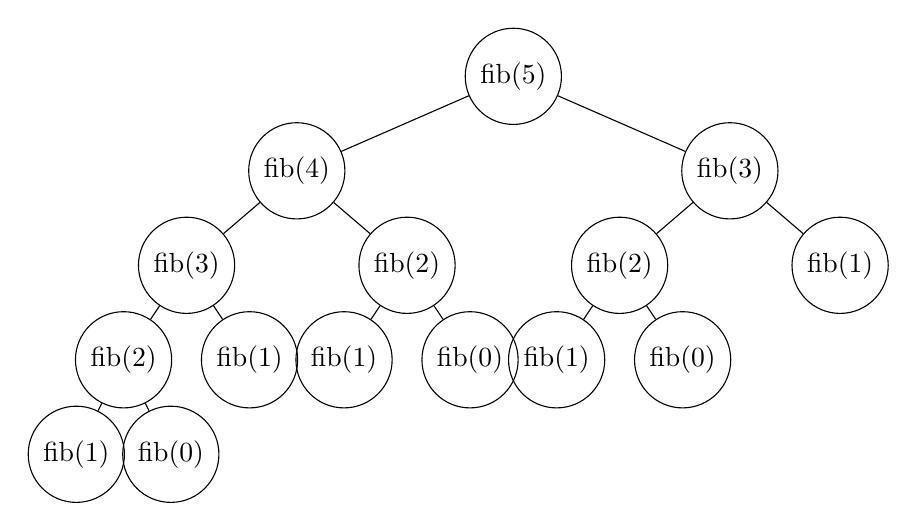
\begin{tikzpicture}[level distance=1.2cm,
  every node/.style={circle,draw,minimum size=8mm},
  level 1/.style={sibling distance=5.5cm},
  level 2/.style={sibling distance=2.8cm},
  level 3/.style={sibling distance=1.6cm},
  level 4/.style={sibling distance=1.2cm}]
\node {fib(5)}
  child {node {fib(4)}
    child {node {fib(3)}
      child {node {fib(2)}
        child {node {fib(1)}}
        child {node {fib(0)}}
      }
      child {node {fib(1)}}
    }
    child {node {fib(2)}
      child {node {fib(1)}}
      child {node {fib(0)}}
    }
  }
  child {node {fib(3)}
    child {node {fib(2)}
      child {node {fib(1)}}
      child {node {fib(0)}}
    }
    child {node {fib(1)}}
  };
\end{tikzpicture}
\end{center}

\textbf{Dynamic programming solution with memoization — Top down approach}

Idea: Cache (memoize) computed results. For any new computation, check cache to see if it holds the result, or else recurse.

\begin{lstlisting}[style=cppstyle]
vector<int> A(n+1, -1); // For memoization
A[0] = 0;
A[1] = 1;

int fibonacci(int n) {
    if (A[n] != -1) // Result in cache
        return A[n];
    else
        A[n] = fibonacci(n-1) + fibonacci(n-2); // Cache result
    return A[n];
}
\end{lstlisting}

\textbf{Dynamic programming solution with tabulation — Bottom up approach}

Idea: Build a table of partial results from the bottom up.

\begin{lstlisting}[style=cppstyle]
int fibonacci(int n) {
    vector<int> A(n+1);
    A[0] = 0;
    A[1] = 1;
    for (int i = 2; i <= n; i++) {
        A[i] = A[i-1] + A[i-2];
    }
    return A[n];
}
\end{lstlisting}

Time: \(O(n)\)  
Space: \(O(n)\)  
Turns out you don't need a whole array. All you need is the last two numbers (two variables). So the space required is only \(O(1)\).

\section{Rod cutting problem}

You are given a rod of size \(n > 0\), it can be cut into any number of pieces \(k\) (\(k \le n\)). Price for each piece of size \(i\) is represented as \(p(i)\) and maximum revenue from a rod of size \(i\) is \(r(i)\) (could be split into multiple pieces). Find maximum \(r(n)\) for the rod of size \(n\).

For example, here’s an array of prices where the array index + 1 indicates rod length:
\[
p = \{1, 5, 8, 9, 10, 17, 17, 20\}
\]

The price of a rod of length 2 is 5.

Example: What is the best price for a rod of length 3?

\begin{itemize}
    \item Break into 3 pieces of length 1: \$3
    \item Break into 1 piece of length 2 and 1 piece of length 1: \$6
    \item Don't break the rod: \$8
\end{itemize}

Best price: don't cut the rod.

Example for rod of length 4: breaking up into 2 and 2 yields \$10.

Let's build some intuition:

\begin{itemize}
    \item Length 1: only possibility price \$1
    \item Length 2: possibilities (1,1)(cut) or (0,2) (uncut) → max(\$2, \$5) = \$5
    \item Length 3: possibilities (0,3), (1,2) → max(\$8,\$6) = \$8
    \item Length 4: (0,4), (1,3), (2,2) → max(\$9,\$9,\$10) = \$10
\end{itemize}

Note how we use the optimal solutions of smaller subproblems, and how the subproblems repeat. 

General algorithm:

\begin{lstlisting}[style=cppstyle]
int rodCutting(const vector<int>& P, int n) {
    vector<int> maxP(n+1, 0);
    for (int i = 1; i <= n; i++) {
        int maxVal = P[i-1];
        for (int j = 1; j <= i/2; j++) {
            maxVal = max(maxVal, maxP[j] + maxP[i-j]);
        }
        maxP[i] = maxVal;
    }
    return maxP[n];
}
\end{lstlisting}

Complexity: \(O(n^2)\)

\section{Max sum of non adjacent elements}

Given an array of positive integers, find the maximum sum of non adjacent elements.

Example: [75, 105, 120, 75, 90, 135]  
Ans: 330 = 75 + 120 + 135

\subsubsection*{Thinking Through the Maximum Sum of Non-Adjacent Elements}

Let us think about the problem step by step:

If we can solve a smaller problem, can we use that to construct the solution of a larger one?

\begin{itemize}
    \item Input: $[75]$ \\
    Best sum: $75$
    
    \item Input: $[75, 105]$ \\
    Best sum: $\max(75, 105) = 105$
    
    \item Input: $[75, 105, 120]$ \\
    If we include $120$, then the best is $75 + 120 = 195$. \\
    If we exclude $120$, the best is $105$. \\
    Thus, $\max(195, 105) = 195$. We would include $120$.
    
    \item Running total so far: $[75, 105, 195]$
    
    \item Next input element: $75$ \\
    Including this $75$: $105 + 75 = 180$ \\
    Excluding: $195$ \\
    Best: $\max(180, 195) = 195$
    
    \item Running total so far: $[75, 105, 195, 195]$
    
    \item Next element: $90$ \\
    Including: $195 + 90 = 285$ \\
    Excluding: $195$ \\
    Best: $285$
    
    \item Running total so far: $[75, 105, 195, 195, 285]$
    
    \item Next element: $135$ \\
    Including: $195 + 135 = 330$ \\
    Excluding: $285$ \\
    Best: $\max(330, 285) = 330$
    
    \item Final maximum sums: $[75, 105, 195, 195, 285, 330]$
\end{itemize}

General approach:

\begin{lstlisting}[style=cppstyle]
int maxSumNonAdj(const vector<int>& in) {
    int n = in.size();
    vector<int> maxSum(n);
    maxSum[0] = in[0];
    maxSum[1] = max(in[0], in[1]);
    for (int i = 2; i < n; i++) {
        maxSum[i] = max(maxSum[i-1], maxSum[i-2] + in[i]);
    }
    return maxSum[n-1];
}
\end{lstlisting}

\section{Levenshtein Distance (Edit distance)}



The Levenshtein distance between two words is the minimum number of single-character edits 
(insertions, deletions, or substitutions) required to change one word to another. Each of these operations has unit cost.

For example, the Levenshtein distance between kitten and sitting is 3. 

\begin{quote}
\texttt{kitten} $\rightarrow$ \texttt{sitten} \hfill (substitute \texttt{k} for \texttt{s}) \\
\texttt{sitten} $\rightarrow$ \texttt{sittin} \hfill (substitute \texttt{e} for \texttt{i}) \\
\texttt{sittin} $\rightarrow$ \texttt{sitting} \hfill (insert \texttt{g} at the end) \\
Total operations = 3
\end{quote}

This problem exhibits \textbf{optimal substructure} — it can be broken down into solving simpler subproblems.

\subsubsection*{Problem Definition}
Given two strings $X[1 \ldots m]$ and $Y[1 \ldots n]$, compute the minimum number of edit operations to convert $X$ into $Y$.

\subsubsection*{Subproblem}
Convert substring $X[1 \ldots i]$ to $Y[1 \ldots j]$ using edit operations.

\subsubsection*{Recursive Cases (Top-Down)}

\begin{description}
  \item[Case 1:] One of the substrings is empty. \\
  If $X$ is empty, insert all remaining characters from $Y$, and vice versa. \\
  \textbf{Example:} $(\texttt{""}, \texttt{"ABC"}) \rightarrow (\texttt{"ABC"}, \texttt{"ABC"})$ \\
  \textbf{Cost:} 3

  \item[Case 2:] Last characters of $X$ and $Y$ match. \\
  No edit needed; recurse on $X[1 \ldots i-1]$ and $Y[1 \ldots j-1]$. \\
  \textbf{Example:} $(\texttt{"ACC"}, \texttt{"ABC"}) \rightarrow (\texttt{"AC"}, \texttt{"AB"})$ \\
  \textbf{Cost:} 0

  \item[Case 3:] Last characters differ — consider three operations and take the minimum:
  \begin{itemize}
    \item \textbf{Delete from $X$:} recurse on $X[1 \ldots i-1]$, $Y[1 \ldots j]$ \\
    \textit{Example:} $(\texttt{"ABA"}, \texttt{"ABC"}) \rightarrow (\texttt{"AB"}, \texttt{"ABC"})$
    
    \item \textbf{Delete from $Y$:} recurse on $X[1 \ldots i]$, $Y[1 \ldots j-1]$ \\
    \textit{Example:} $(\texttt{"ABA"}, \texttt{"ABC"}) \rightarrow (\texttt{"ABA"}, \texttt{"AB"})$
    
    \item \textbf{Substitute:} recurse on $X[1 \ldots i-1]$, $Y[1 \ldots j-1]$ \\
    \textit{Example:} $(\texttt{"ABA"}, \texttt{"ABC"}) \rightarrow (\texttt{"ABC"}, \texttt{"ABC"})$
  \end{itemize}
\end{description}

\subsubsection*{Recurrence Relation}

\[
\text{dist}[i][j] =
\begin{cases}
\max(i, j) & \text{if } \min(i, j) = 0 \\
\text{dist}[i-1][j-1] & \text{if } X[i] = Y[j] \\
1 + \min\{\text{dist}[i-1][j], \text{dist}[i][j-1], \text{dist}[i-1][j-1]\} & \text{if } X[i] \neq Y[j]
\end{cases}
\]

\subsubsection*{Time Complexity}
\[
\mathcal{O}(mn)
\]
where $m$ and $n$ are the lengths of strings $X$ and $Y$. Brute-force approaches are exponential, but dynamic programming reduces this to polynomial time.

\begin{table}[h!]
\centering
\begin{tabular}{c|cccccccc}
  &   & s & i & t & t & i & n & g \\
\hline
  & 0 & 1 & 2 & 3 & 4 & 5 & 6 & 7 \\
k & 1 & 1 & 2 & 3 & 4 & 5 & 6 & 7 \\
i & 2 & 2 & 1 & 2 & 3 & 4 & 5 & 6 \\
t & 3 & 3 & 2 & 1 & 2 & 3 & 4 & 5 \\
t & 4 & 4 & 3 & 2 & 1 & 2 & 3 & 4 \\
e & 5 & 5 & 4 & 3 & 2 & 2 & 3 & 4 \\
n & 6 & 6 & 5 & 4 & 3 & 3 & 2 & 3 \\
\end{tabular}
\caption{Levenshtein Distance Matrix for \texttt{kitten} and \texttt{sitting}. Edit distance = 3}
\end{table}

\section{Knapsack problem (1/0)}

\textbf{Optimization Problem}

\textbf{Input:}
\begin{itemize}
    \item $n$ items, each with:
    \begin{itemize}
        \item value $V_i$ (non-negative)
        \item weight $W_i$ (non-negative, integral)
    \end{itemize}
    \item capacity $W$ (a non-negative integer)
\end{itemize}

\textbf{Output:} Select a subset of items that maximizes the total value without exceeding the capacity $W$.

\subsubsection*{Bottom-Up Dynamic Programming Approach}
We define a DP table $V[i][j]$ to represent the maximum value achievable using the first $i$ items and capacity $j$. We construct this table using the recurrence:

\begin{itemize}
    \item \textbf{Case 1:} Skip the $i$-th item
    \[
    V[i][j] = V[i-1][j]
    \]
    
    \item \textbf{Case 2:} Include the $i$-th item, provided $j \geq W_i$
    \[
    V[i][j] = V[i-1][j - W_i] + V_i
    \]
    
    \item \textbf{Final recurrence:}
    \[
    V[i][j] = \max(V[i-1][j],\ V[i-1][j - W_i] + V_i)
    \quad \text{(if } j \geq W_i\text{)}
    \]
    
    \item \textbf{Boundary conditions:}
    \[
    V[0][j] = 0 \quad \text{(no items)} \\
    V[i][0] = 0 \quad \text{(zero capacity)}
    \]
\end{itemize}

\textbf{Time Complexity:} $\mathcal{O}(nW)$, where $n$ is the number of items and $W$ is the maximum knapsack capacity (assumed to be an integer).
Given items with values \(V_i\) and weights \(W_i\), capacity \(W\), maximize value without exceeding \(W\).

\begin{lstlisting}[style=cppstyle]
int knapsack(const vector<int>& V, const vector<int>& W, int capacity) {
    int n = V.size();
    vector<vector<int>> dp(n+1, vector<int>(capacity+1, 0));
    for (int i = 1; i <= n; i++) {
        for (int w = 0; w <= capacity; w++) {
            if (W[i-1] <= w)
                dp[i][w] = max(dp[i-1][w], dp[i-1][w - W[i-1]] + V[i-1]);
            else
                dp[i][w] = dp[i-1][w];
        }
    }
    return dp[n][capacity];
}
\end{lstlisting}

Complexity: \(O(nW)\)

\subsection*{Example:}
W = 6 \\
v1 = 3, w1 = 4 \\
v2 = 2, w2 = 3 \\
v3 = 4, w3 = 2 \\
v4 = 4, w4 = 3 \\

\begin{table}[h!]
\centering
\begin{tabular}{c|ccccccc}
\textbf{Items} $\backslash$ \textbf{Weights} & 0 & 1 & 2 & 3 & 4 & 5 & 6 \\
\hline
0 & 0 & 0 & 0 & 0 & 0 & 0 & 0 \\
1 & 0 & 0 & 0 & 0 & 3 & 3 & 3 \\
2 & 0 & 0 & 0 & 2 & 3 & 3 & 3 \\
3 & 0 & 0 & 4 & 4 & 4 & 6 & 7 \\
4 & 0 & 0 & 4 & 4 & 4 & 8 & 8 \\
\end{tabular}
\caption{Value matrix for 0/1 Knapsack Problem. Rows represent items and columns represent weight capacities.}
\end{table}

To figure out which items were included in the knapsack, backtrack

Start from the lower right corner V[4][6]

Was this value gotten from taking or not taking item 4? Since V[3][6] != V[4][6], item 4 was chosen.

V[4][6] was obtained from V[3][3] (Subtracting weight of item 4)

Again V[3][3] != V[2][3], so item 3 was chosen.

V[3][3] was obtained from V[2][1] (subtracting weight of item 3)

Since V[2][1] has no residual capacity to include any more items, search terminates.



\section{More Examples}

See: \url{https://www.techiedelight.com/Category/dynamic-programming/}

\end{document}